
\section{Overview of Hyperdynamics}
\index{hyperdynamics!TAD}
\index{hyperdynamics!BPD}
\index{temperature accelerated dynamics (TAD)|see{hyperdynamics, TAD}}
\index{bias potential dynamics (BPD)|see{hyperdynamics, BPD}}
The first thing to note about the hyperdynamics methods in
\D{} is that they were designed for studies of kinetic processes in 
the solid state, which mostly means diffusion. In solids diffusion is
characterised by infrequent atomic `hops' occurring on a time scale of
order 100 ps to 1000 ps per hop, which is too infrequent to give a
measurable diffusion in a normal molecular dynamics
simulation. Hyperdynamics methods are designed to overcome this
problem by accelerating the hopping frequency.

The hyperdynamics methods built into \D{} are {\em Bias Potential
Dynamics} (BPD) \cite{voter-97a} and {\em Temperature Accelerated
Dynamics} (TAD) \cite{voter-00a}, both of which were conceived by
Voter {\em et al}, though the implementation of BPD in the program
uses the bias potential devised by Hamelberg, Mongan and McCammon
\cite{hamelberg-04a}, which is simpler to use. 
In passing it is useful to note that BPD can be used to improve
configurational sampling in systems other than solids and this
facility has been retained in the \D{} implementation (see section
\ref{cfgdyn}).

\begin{figure}[ht]
\hrule
\vspace{1.0cm}
\begin{center}
\centerline{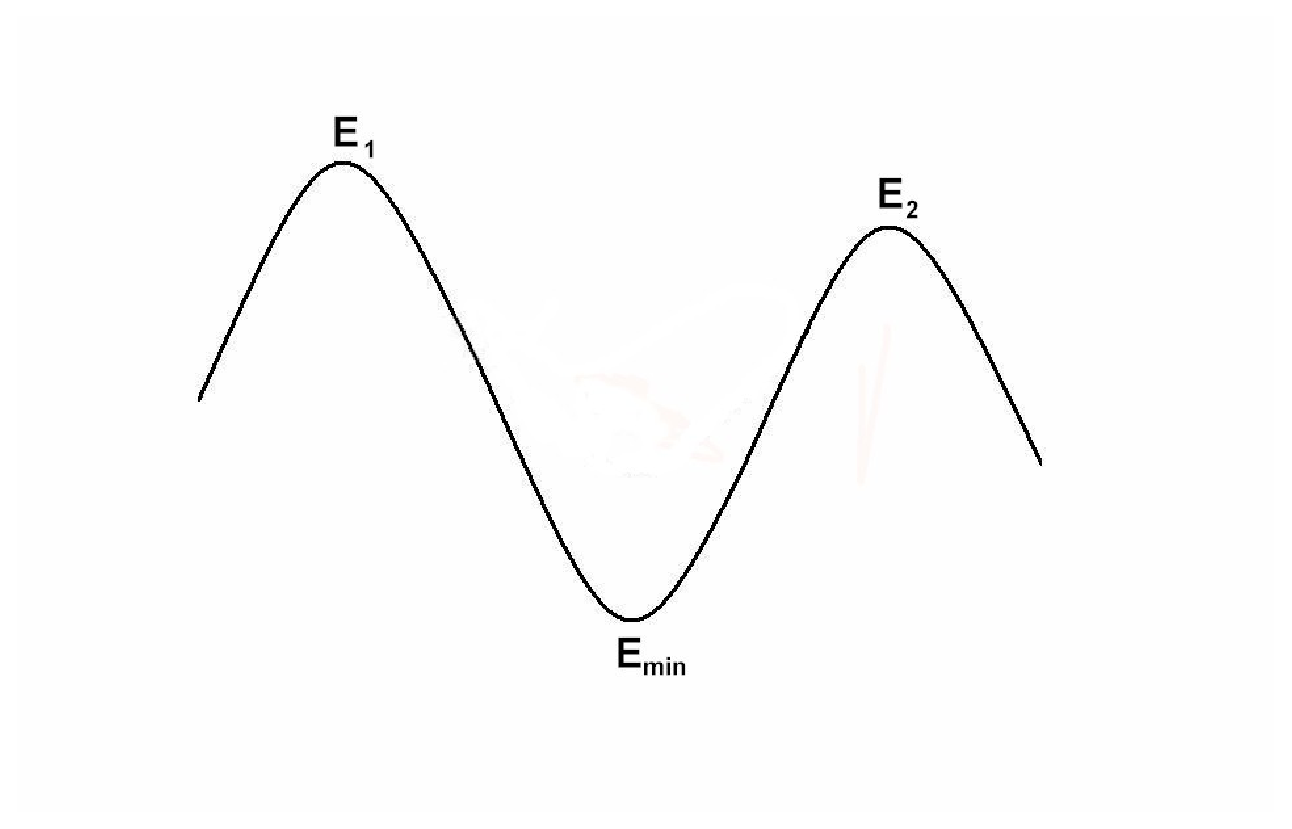
\psfig{file=Hills.ps,height=6.0cm}}
\end{center}
\caption{Model Potential Energy Surface.\label{potsurf}}
The potential energy surface of a solid is characterised by deep
energy basins, such as $E_{min}$, representing the various structural
states. Escape to other states (i.e. diffusion) must go via `saddle
points' on the surface indicated by points $E_{1}$ and $E_{2}$. The
energy differences ($E_{1}-E_{min}$) or ($E_{2}-E_{min}$) represent
the activation energies ($E^{*}$) required to enable escape via the
respective saddle points. Thermal excitation alone is insufficient to
achieve escape in a reasonable time.

~
\hrule
\end{figure}

The basic problem in simulating diffusion in solids is that each
possible structure of the system is trapped in a deep basin in
the potential energy surface (see figure \ref{potsurf}) representing a
particular `state'. For diffusion to occur the system must become
sufficiently thermally excited to achieve the activation energy
$E^{*}$ necessary to escape.  In dimensions higher than 1, $E^{*}$
represents a `saddle point' on the potenial energy surface.  Special
techniques are required to accelerate the escape and achieve a
measurable diffusion in a reasonable time. These however must be
devised so that the kinetic processes of the original system may be
faithfully reconstructed. Both the BPD and TAD methods in \D{}, which
are respectively described in sections \ref{BPD} and \ref{TAD} below,
satisfy this requirement.

It is apparent from the discussion above that an important requirement
in hyperdynamics is the calculation of the activation energy, which is
equivalent to determining the saddle point between two states. This is
accomplished in \D{} by a technique known as the `Nudged Elastic Band'
(NEB) method. Understanding the NEB method is a prerequisite for using
the \D{} hyperdynamics methods correctly, so a description of it is
given in the following section.

\section{The Nudged Elastic Band Calculation}
\index{hyperdynamics!NEB}
\index{nudged elastic band (NEB)|see{hyperdynamics, NEB}}

\label{NEB}
\begin{figure}[ht]
\hrule
\vspace{1.0cm}
\begin{center}
\centerline{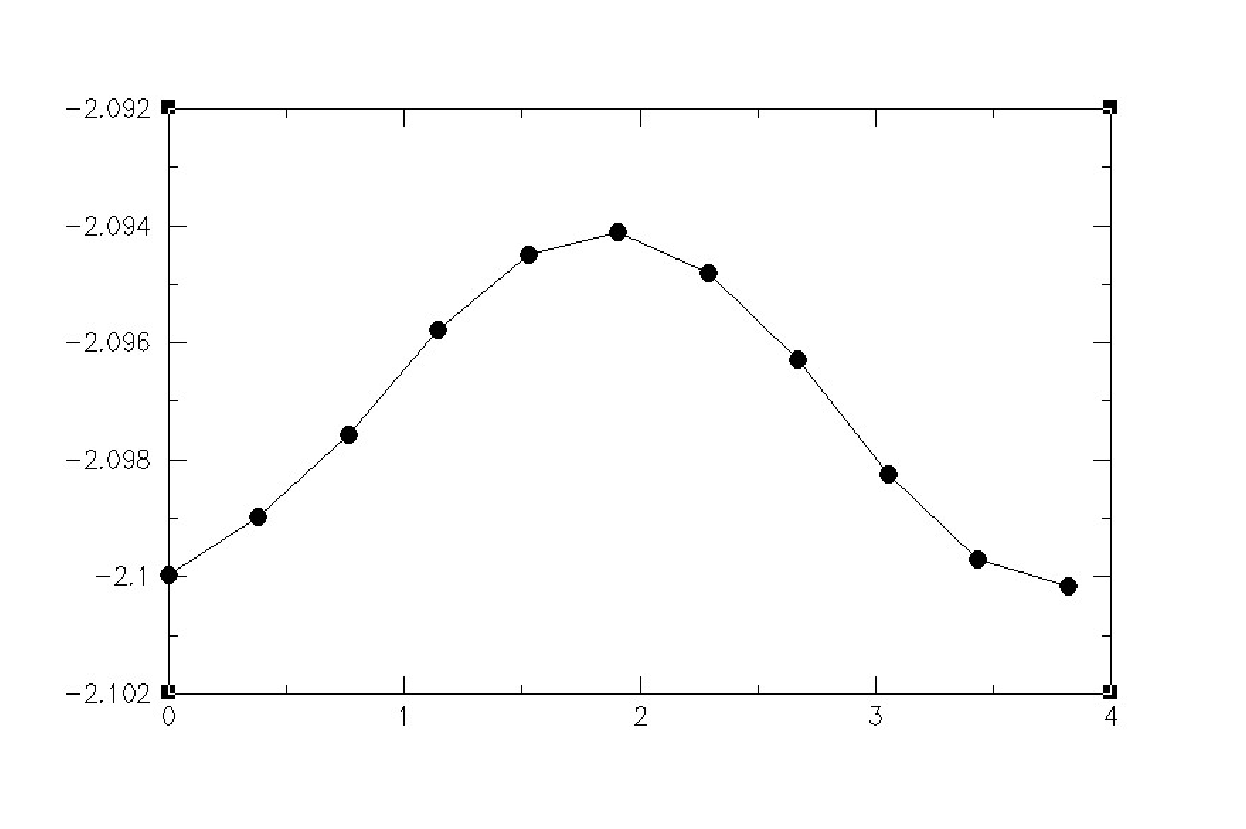
\psfig{file=NEB.ps,height=5cm}}
\end{center}
\caption{Basic NEB Theory\label{nebfig}}
\index{hyperdynamics!reaction path}
Plot of bead configuration energy vs. reaction path for a NEB
calculation of a structural transition in a Lennard Jones solid.

~
\hrule
\end{figure}
The `Nudged Elastic Band' (NEB) method is a standard method for
determining the energy optimised pathway between two known
structures. In \D{} it is used to find the escape pathway (also called
the `reaction path') \index{hyperdynamics!reaction path} between
structural basins, yielding the activation energy in the process. The
implementation is based on the method described by Henkelman and
Jonsson\cite{henkelman-00a} though it has been adapted to work in
parallel. The method is as follows.

\begin{enumerate}
\item The start and end points of the NEB construction are the energy
minimised structures for states A and B. (A structure ($\vek{R}^{N}$) is
defined as the set of $3N$ coordinates locating all $N$ atoms in the system.)
\item A series of states is constructed by linear interpolation between the
structures of states A and B i.e. a series of configurations
$\vek{R}^{N}_{i}$ is generated with $i=0,\ldots,N_{neb}$ such that $i=0$
indicates state A and $i=N_{neb}$ indicates state B and
\begin{equation}
\vek{R}^{N}_{i}=\vek{R}^{N}_{0}+(i/N_{neb})*(\vek{R}^{N}_{N_{neb}}-\vek{R}^{N}_{0})
\end{equation}
For convenience these configurations are called the `beads' of the NEB
`chain'. Each bead has a configuration energy which may be written as
$V_{c}(\vek{R}^{N}_{i})$. This is the usual configuration energy for a
system with an atomic structure $\vek{R}^{N}_{i}$.
\item Each bead in the NEB chain  is then connected to its two 
nearest neighbours by a harmonic spring (except for the end beads which
have only one neighbour each), so that the beads make a chain strung 
from state A to state B. The spring energy of the whole chain is 
then defined as
\begin{equation}
V_{s}(\vek{R}^{N}_{N_{neb}})=\frac{1}{2}k_{neb}\sum_{i=1}^{N_{neb}}(\vek{R}^{N}_{i}-\vek{R}^{N}_{i-1})^{2}
\end{equation}
where $k_{neb}$ is the spring force constant.
\item With the chain thus defined, the objective is now to minimise
the energy function $E(\vek{R}^{N}_{N_{neb}})$ where
\begin{equation}
E(\vek{R}^{N}_{N_{neb}})=V_{s}(\vek{R}^{N}_{N_{neb}})+\sum_{i=1}^{N_{neb}-1}V_{c}(\vek{R}^{N}_{i})
\end{equation}
in which the adjustable variables are the configurations $\vek{R}^{N}_{i}$
(i.e. the atomic coordinates in each structure), while the chain end
beads at $\vek{R}^{N}_{0}$ and $\vek{R}^{N}_{N_{neb}}$ remain fixed.
\item It is clear that the unconstrained configurations $\vek{R}^{N}_{i}$ would
normally relax into the nearest local minimum, but that this cannot
happen if they are sufficiently constrained by the harmonic springs
(i.e. $k_{neb}$ is strong enough). Thus the minimisation of the chain
will tend to locate each bead in a position along a path between
states A and B like a stretched necklace, which approximates the
minimum energy path between the two states.
\item In practice this simple idea needs refining (or
`nudging'). Thus care is taken to ensure that the springs forces
acting on the beads and the forces optimising bead configurations are
approximately orthogonal. This means that the atomic forces are zeroed
in directions parallel to the path of the chain and the spring forces
are zeroed in directions normal to the chain. The method of Henkelman
and Jonsson \cite{henkelman-00a} is designed to achieve this.
\item If the NEB optimisation works correctly, the result will be that
beads are evenly spaced along the minimum energy path (see figure
\ref{nebfig}). Then by fitting the energies of the beads as a function
of the distance along the path, the maximum energy (i.e. $E^{*}$)
along the path may be obtained. The \D{} NEB routine does this fit using
third order splines.
\end{enumerate}

\section{Bias Potential Dynamics}
\label{BPD}
\subsection{Theory of Bias Potential Dynamics}
\begin{figure}[ht]
\hrule
\vspace{1.0cm}
\begin{center}
\centerline{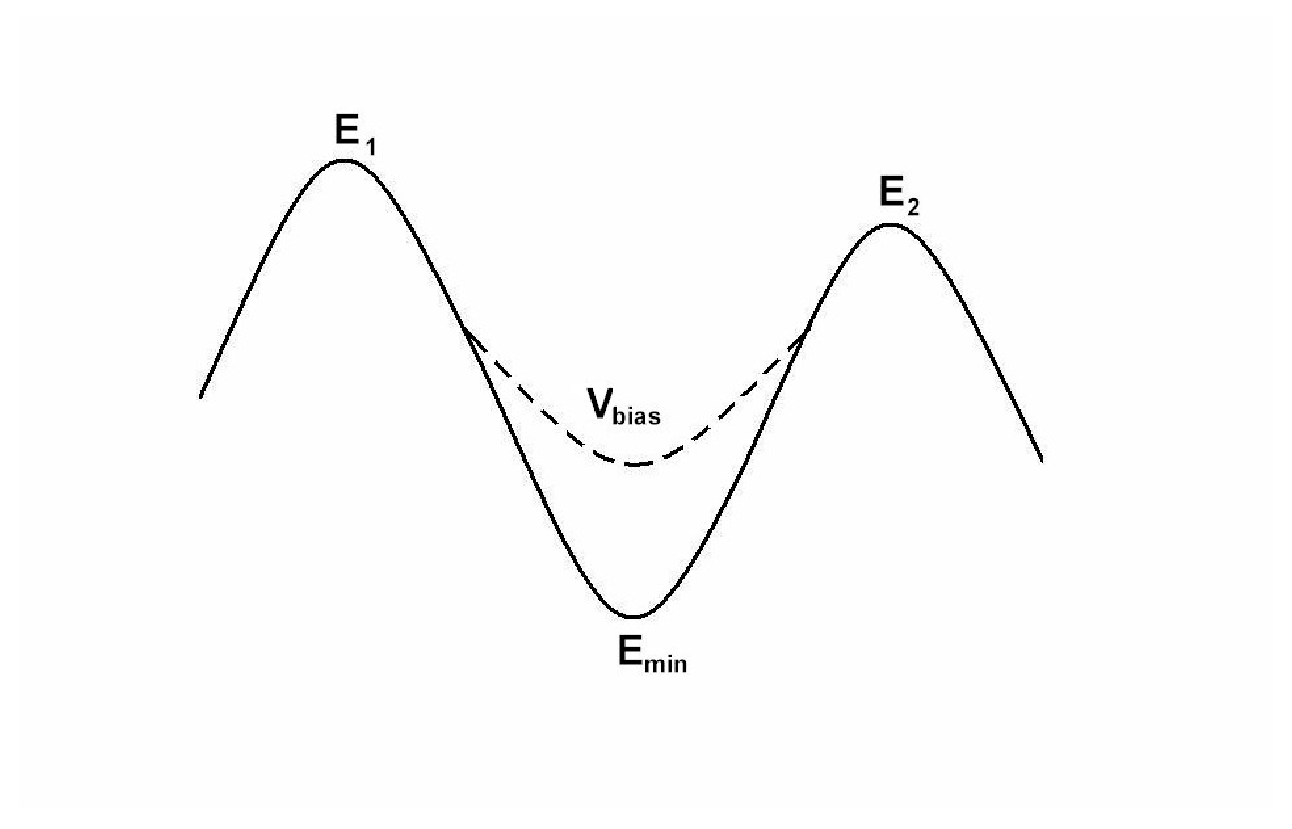
\psfig{file=BiasPot.ps,height=6cm}}
\end{center}
\caption{Basic BPD Theory\label{bpdfig}}
The normal potential energy surface (continuous line) is characterised
by deep basins such as $E_{min}$ from which escape is improbable. The
biased potential $V_{bias}$ (dashed line) reduces the basin depth,
making transitions more likely. To preserve the kinetic pathway of the
original system, the bias potential must be less than the saddle
points $E_1$ and $E_2$ and for molecular dynamics purposes ideally should
join continuously to the normal system potential (see text).

~
\hrule
\end{figure}
\index{hyperdynamics!BPD}
BPD works on the simple principle that the addition of a suitable
potential term to original system potential can have the effect of
reducing the depth of the potential basin (see figure \ref{bpdfig}) so
assisting escape to neighbouring states. The biased system potential
($V_{bias}(\vek{R}^{N})$) is thus given by
\begin{equation}
V_{bias}(\vek{R}^{N})=V(\vek{R}^{N})+W_{bias}(\vek{R}^{N}) \label{sbias}
\end{equation}
where $V(\vek{R}^{N})$ is the original system potential and
$W_{bias}(\vek{R}^{N})$ is the bias potential.
Voter \cite{voter-97a} has shown that using a bias potential
accelerates the diffusion rate constant $k^{TST}$ (as defined by
Transition State Theory) by a boost factor:
\begin{equation}
 k^{TST}_{bias}=\left <e^{\beta W_{bias}(\vek{R}^{N})}\right
 >_{bias} k^{TST} \label{boost}
\end{equation}
where $\beta=1/k_BT$ and the ensemble average, which is calculated in the
biased system, represents the boost factor.

However this simple accelerative factor alone is not sufficient if a
faithful description of the diffusion path in the original system is
required. Voter \cite{voter-97a} showed that to recover the true
diffusional path it is important that the bias potential does not
affect the structure of the transition state (i.e. the saddle points
for the system potential energy surface). If this is the case
then the {\em relative} rate constants for escape from a given structure (or
state) to any other neighbouring state remains constant i.e. for
transitions from state A to state B or state C:
\begin{equation}
\frac{k^{TST}_{A_{b}\rightarrow B}}{k^{TST}_{A_{b}\rightarrow C}}=
\frac{k^{TST}_{A\rightarrow B}}{k^{TST}_{A\rightarrow C}} \label{votcon}
\end{equation}
where $A_{b}$ represents state A simulated with the bias potential
present.  With this condition satisfied for all possible transitions a
simulation will reproduce the diffusional path obtained in the
original system, but at an accelerated rate.

An early difficulty with BPD was defining the bias potential. However
a particularly convenient form has been devised by Hamelberg {\em et
al} \cite{hamelberg-04a} which has the form
\begin{equation}
W_{bias}(\vek{R}^{N})=H(E_{bias}-V(\vek{R}^{N}))
\frac{[E_{bias}-V(\vek{R}^{N})]^{2}}
{[\alpha+E_{bias}-V(\vek{R}^{N})]}, \label{vbias}
\end{equation}
where $\alpha$ is a constant that controls the curvature of
the bias potential (see below). $E_{bias}$ is a fixed potential energy
level above which the bias potential $W_{bias}(\vek{R}^{N}))$ becomes
zero (and the unbiased potential is restored). This is controlled by
$H(x)$, a Heaviside function, which is zero if the argument $x<0$ and
1 if $x>0$. Thus setting $E_{bias}$ correctly provides a means to
preserve the structure of the saddle points of the original
surface. (Note however that the user must determine a safe value for
this.) A value of $E_{bias}$ set above the value of the activation
energy $E^{*}$ anywhere on the surface invalidates Voter's condition
(\ref{votcon}).

Using the definition of the bias potential (\ref{vbias}) it is easy to
show that the atomic forces in the biased system are given by:
\begin{equation}
\vek{f}_{i}^{bias}=\vek{f}_{i}\left 
(\frac{\alpha}{\alpha+E_{bias}-V(\vek{R}^{N})}\right )^{2}~~~~~~~~~E_{bias}>V(\vek{R}^{N}).
\end{equation}
When $E_{bias}\le V(\vek{R}^{N})$ the atomic forces are the same as
for the unbiased system.

The constant $\alpha$ in equation (\ref{vbias}) plays an important role. If it
is set to zero then $V_{bias}(\vek{R}^{N})=E_{bias}$ i.e. the biased system
potential (\ref{sbias}) becomes a flat surface within the basins of the
original potential energy surface. In this case BPD is equivalent to a
technique known as ``puddle skimming'' \cite{rahman-02a}, which is a viable
method for Monte Carlo simulation, but has a disadvantage for molecular
dynamics in that whenever $E_{bias}=V(\vek{R}^{N})$ the atomic forces become
discontinuous. For dynamics a nonzero value of $\alpha$ is therefore always to
be preferred. Hamelberg {\em et al} \cite{hamelberg-04a} give the following
prescription for obtaining $\alpha$.

Firstly the system is simulated under normal conditions at the
required state point and the mean value for the system configuration
energy is determined. This average value is referred to as $V_{min}$
and is used to represent the minimum configuration energy. Then a
value of $E_{bias}$ is chosen that is able to to provide a suitable
boost factor (as in equation \ref{boost}). $\alpha$ is then defined to
be
\begin{equation}
\alpha=E_{bias}-V_{min.}
\end{equation} 
This prescription gives a system bias potential (\ref{sbias}) which is
everywhere differentiable (with continuous forces) and usefully
retains some semblance of the shape of the original potential energy
surface. The user is at liberty to chose any value
$E_{bias}>V_{min}$, which is useful for configurational
sampling, but for hyperdynamics satisfying the Voter condition
(\ref{votcon}) $E_{bias}$ must not exceed the system configuration
energy at any saddle point representing an escape route from a
potential basin.

Finally it should be noted that simulations performed under the
influence of a bias potential naturally do not return system averages
corresponding to the thermodynamic state of the original system
at the specified temperature and pressure. The calculation of the true
thermodynamic averages requires a correction in the form of a {\em
weighted average} \cite{hamelberg-04a}. The true thermodynamic average
$<A>$ of a property $A$ is thus given by
\begin{equation}
<A>=\frac{<Ae^{\beta W_{bias}(\vek{R}^{N})}>_{bias}}
{<e^{\beta W_{bias}(\vek{R}^{N})}>_{bias}} \label{cbias}
\end{equation}
Where the ensemble averages are obtained in the biased system.  When
running the BPD options \D{} calculates all system averages in this way.

\subsection{Running a BPD Simulation}

Two ways of running bias potential dynamics are available in \D{}. The
first is referred to as ``Full Path Kinetics'' since it attempts to
reproduce a full description of the diffusion path with the associated
activation energies. This is described in section \ref{FPK}. The
second is ``configurational sampling'', which exploits BPD to explore
the range of structural states available to a system, which need not
necessarily be in the solid state. It may also be used to improve
thermodynamic averaging of a system at a given temperature, where
equilibration is problematical due to long time scales. This is
described in section \ref{cfgdyn}.

\subsection{Full Path Kinetics}
\label{FPK}
\index{hyperdynamics!BPD!full path kinetics}
This option is intended to determine the true diffusional path that a
solid state system follows at a given temperature, but at an
accelerated rate.  Each time the system transforms from one structure
to another (i.e. from one state to another) the program records the
states it encounters and calculates both the activation energy $E^{*}$
associated with the transition and extrpolates the time at which the
transition would have occured in the unbiased system.  This information may
subsequently be used to determine the full kinetics of the system.

The method in outline is as follows. 
\begin{enumerate}
\item The first operation of the program is to construct a reference 
state for the structure by energy minimisation.
The simulation then proceeds with the biased potential option in much
the same manner as a normal simulation, but during which a running
estimate of the boost factor (in equation (\ref{boost})) is computed. 
\item At user defined intervals (called here a `BPD block') the 
simulation is halted and the structure energy minimised to create new
reference structure, which is compared with the original reference
state to determine if a transition has occurred. A transition is
deemed to have occured if one or more atoms are displaced by more than
a preset distance (the `catch radius').  If a transition is
detected, a NEB calculation is initiated, using the two reference
structures, to find the activation energy ($E^{*}$). 
\item A determination of the time of the transition is made.
In \D{} the occurrence time of the transition ($t_{occ}$) is determined
by checking back from the detection of the transition through past
configurations saved at regular intervals (which should be much less
than a BPD block).  Each saved configuration is energy minimised and
compared with the reference state structure until the first occurrence
of the new state is found. This provides a reasonable accuracy on the
transition time, somewhat better than using the end time of the BPD
block in which the transition occurred. The transition time is
then corrected for the boost factor in equation (\ref{boost}).
\item The new found state becomes the reference state for the next stage of
the simulation. If no transition was detected the original reference state is
left in place.  In both cases the simulation continues
from the end of the block as if uninterrupted. (Note this 
is markedly different from the TAD procedure
described in section \ref{TAD}.)
\item The simulation is continued until, from inspection, it apparent 
that all significant kinds of transition have been observed. When this
is is anybody's guess, but clearly some knowledge of the system,
gained from other sources, it invaluable here.
\item With all the information gathered it should now be possible to 
determine the full diffusion process for the original system at the
state point chosen.
\end{enumerate}

The recommended procedure for running BPD with \D{} is as follows.
\begin{enumerate}
\item Run a normal (unbiased) simulation of the system at the required
state point (temperature and volume). Make sure the system does not
undergo any structural changes that nullify the validity of the BPD
approach (e.g. melting). Record the average configuration energy
($V_{min}$) of the system. Keep the REVCON file to use as the starting
CONFIG structure for the BPD simulation.
\item Set up the BPD option in the CONTROL file as follows:
\begin{enumerate}
\item Set the {\bf bpd path} directive.
\item Define the energy units for the BPD parameters e.g. \newline
      {\bf units} {\em s}\newline where {\em s} is one of {\em eV,
      kcal, kJ or K}, signifying electron volts, kilo cals per mole,
      kilo joules per mole or Kelvin, respectively. No {\bf units}
      directive means DL\_POLY internal units apply. Forces are given 
      in chosen energy units per Angstrom.
\item Set the value of the average potential ($V_{min}$) e.g.\newline
      {\bf vmin} {\em f} \newline
      where {\em f} is the known average potential.
\item Set the value of the potential bias ($E_{bias}$) e.g. \newline
      {\bf ebias} {\em f} \newline
      where {\em f} is the bias energy level.
\item Set the size of the simulation BPD block i.e. the number of time steps
      between structure optimisations (for transition
      detection). e.g. \newline {\bf num\_block} 500.
\item Set the number of configurations between each write of a tracking
      configuration file. This should be an integer divisor of the BPD
      block number. e.g. \newline
      {\bf num\_track} 10.
\item Set the `catch radius' i.e. the minimum distance 
      in Angstroms any atom may be displaced in the minimised structure 
      before it is recorded as a transition e.g. \newline 
      {\bf catch\_radius} 3.0.
\item Set the NEB spring constant (in specified energy units per $\AA^2$). 
       e.g. \newline {\bf neb\_spring} 1000.0 (for DL\_POLY units).
\item Select a minimisation option.  e.g. 
      \newline {\bf force} {\em key tol}.\newline 
      Where {\em key} is one of {\em force, energy, position} and {\em
      tol} is the convergence tolerance.
      (The recommended choice is {\em force} with a tolerance 
      of 1.0 in DL\_POLY units.)
\item Close the BPD definition with the directive \newline
      {\bf endbpd}
\end{enumerate}
\item Set other CONTROL file directives as follow:
\begin{enumerate}
\item Select the {\bf restart noscale} option if the CONFIG file was
      pre-equilibrated, otherwise leave out the {\bf restart} keyword 
      altogether.
\item Set the length of the simulation required ({\bf steps}) and the 
      equilibration period ({\bf equil}) (both in time steps). The
      equilibration can be short if the system was pre-equilibrated.
\item In setting the job {\bf close time}, it is
      recommended to set the number to at least 500 times the clock
      time it takes to do one normal MD time step. This is to prevent
      the program running out of time during a structural
      minimisation. The timing information for this may be taken from
      the previous equilibration run.
\item Set the remaining CONTROL keywords as were defined for the initial
      equilibration simulations.
\end{enumerate}
\item Before starting the BPD simulation, use the UNIX `mkdir' command to
      make the following empty directories: 
\begin{itemize}
   \item {\em BASINS} - to receive any new structures found;
   \item {\em TRACKS} - to store the tracking configurations;
   \item {\em PROFILES} - to store any transition pathways found by
   NEB calculations.
\end{itemize}
   If the directories {\em BASINS, TRACKS} and {\em PROFILES} already
   exist then carefully archive the data before deleting the
   contents. These directories should not be emptied if the simulation
   is continuing (restarting) and a full history of the kinetics is
   required. More about these directories and the files they contain
   can be found in section \ref{hypfiles}
\item Run the BPD simulation. This will perform a simulation at the
   state point requested, checking for structural transitions at the
   BPD block intervals specified. Each time it finds a structural
   transition, it will record the new state, determine the activation
   energy by the NEB method and the (unbiased) transition time using
   the boost factor in equation (\ref{boost}), and then continue the
   simulation.
\item When the simulation ends, proceed as follows.
\begin{enumerate}
\item Check the EVENTS file to see if any structural
  transitions have been obtained. Each event is represented by a
  single record and transitions are flagged with the keyword TRA at
  the start of the record. Use unix `grep' to locate these entries. No
  observed transitions indicates that either a longer simulation is
  necessary, or running with a higher bias $E_{bias}$ should be
  considered.
\item {\bf Important.} If any of the reported transitions has a system
  activation energy that is below $E_{bias}$
  (i.e. $N*E^{*}<E_{bias}-V_{min}$, where $N$ is the number of atoms in the
  system\footnote{Assuming just one atom undergoes the transition!}) this
  represents a violation of the condition in equation (\ref{votcon}), which
  means the observed diffusion path is not a valid representation of the
  original system. The simulation should be repeated with a lower value of
  $E_{bias}$.
\item If the required number of time steps has not been reached, the
  simulation can be restarted from the REVCON, REVIVE and HYPRES files
  (renaming them as CONFIG, REVOLD and HYPOLD for the purpose), and
  setting the directive {\bf restart} (with no qualifier) in the CONTROL
  file.
\item Use the DL\_POLY Java GUI to plot the system energy and temperature
  for the whole of the simulation. Apart from the equilibration
  period, these should hold their values within normal thermodynamic
  fluctuation, even if transitions have occured. If they do not, the
  system has probably not been equilibrated adequately to begin with,
  in which case the simulation should be started again.
\item Check that all the new states the program found are present in 
  the {\em BASINS} directory. Examine them using the DL\_POLY Java
  GUI. There may be signs of imperfect minimisation (atoms not quite
  on lattice sites etc) but this is not a problem in this instance.
  More accurate NEB calculations can be performed later (see section
  \ref{tidyup}) .
\item Check that the profiles for all the reported transitions have been
  written in the {\em PROFILES} directory. These record the change in
  configuration energy as a function of reaction coordinate (or
  diffusion path). 
  Plot these using the DL\_POLY Java GUI. Use the GUI `spline' option
  to get a better idea of what the profiles look like. Take special
  note of any double (or multiple) maxima. The transition is
  considered to end at the first minimum in these cases. It follows
  that the activation energy for the second peak is not available in
  this case, but it can be obtained later by running the NEB facility
  independently for the states concerned (see section \ref{tidyup}).
\item It is useful to determine which atoms have relocated during a
  transition. The program bsncmp.f in the {\em  utility} directory 
  may be used for this purpose. It is designed to compare start and 
  end configurations in the {\em BASINS} subdirectory and list the 
  atoms that have changed location.
\end{enumerate}
\end{enumerate}

\subsection{Things to Be Aware of when Running  Full Path Kinetics BPD}

\begin{enumerate}
\item Choose the `catch radius' carefully, where possible basing it on
  nearest neighbour distances obtained from the parent crystal. A
  consequence of using too large a catch radius is that transitions
  that require a short hop in atom positions may be missed during a
  run. Such misses make it difficult to reconstruct the reaction path
  and, in particular, cause the NEB calculation to crash, since there
  is no simple path between the reference structures.
\item Note that in a BPD simulation the reference state is replaced
  whenever a new state is found. In this respect the reference state
  `follows' the diffusion path. This is a clear distinction from TAD.
\item We repeat again the important message that if any of the 
  transitions reported by PBD has an activation energy that is below
  the value of the bias term $E_{bias}$
  (i.e. $N*E^{*}<E_{bias}-V_{min}$,) this represents a violation of the
  condition in equation (\ref{votcon}), which means the observed
  diffusion path is not a valid representation of the original
  system. The simulation should be repeated with a lower value of
  $E_{bias}$.
\end{enumerate}

\subsection{Exploring Configurational Space}
\label{cfgdyn}
\index{hyperdynamics!BPD!exploring configuration space}
Running \D{} under the BPD option is useful for simply exploring
configurational space. This has a number of uses:
\begin{enumerate}
\item Equilibration at a given temperature is quicker and
 thermodynamic averages can be obtained with greater reliability;
\item It is possible to observe configurations which are
 difficult to obtain under normal conditions, perhaps because they are
 far from the starting state and the system has slow relaxation
 times. Such configurations may be important from a mechanistic
 viewpoint;
\item The trajectory of the system evolves faster, which means that
 movies of the simulation can show the motions of the system on a
 reasonable time scale.
\end{enumerate}

\noindent This option is activated in the CONTROL file by using the 
single-line directive:

{\bf bpd dyn} $f_1$ $f_2$ $s$ 

\noindent where $f_1$ is the value of the required bias ($E_{bias}$), 
$f_2$ is the required value of the operating potential minimum
($V_{min}$) and {\em s} is one of {\em eV, kcal, kJ or K}, signifying
the energy unit of the values entered.

This option runs like a normal \D{} simulation, except that the
system potential is now the biased potential. Consequently average
system properties are calculated using equation (\ref{cbias}). 

It is recommended that the simulation be run with the {\bf traject}
option activated in the CONTROL file so that a HISTORY file is
produced. This may be further analysed to reveal conformational
properties or viewed as a movie (with appropriate software).

\section{Temperature Accelerated Dynamics}
\label{TAD}
\subsection{Theory of Temperature Accelerated Dynamics}

\index{hyperdynamics!TAD}
Temperature Accelerated Dynamics (TAD) was devised by Voter {\em et al}
\cite{voter-00a}. Like BPD it is also a combination of molecular
dynamics and Transition State Theory (TST) for first order processes.
TAD works on the principle that while diffusion in the solid state at
a low temperature is often too slow to measure, at a higher
temperature it may be many orders of magnitude faster. However it is
normally the case that at different temperatures a system will
evolve via different diffusion pathways. So to exploit the
temperature acceleration successfully special care must be taken to
preserve the true mechanistic pathway at the required (low)
temperature. This is precisely what TAD does.

An appropriate model for a first order diffusion process supposes a
system trapped in a potential basin (state A), from which it may
escape through thermal excitation to a new state (state B). If the
system is created in state A at time zero, the probablity of it being
found in the same state at a later time $t$ is
\begin{equation}
P(t)dt=k \exp(-k t) dt
\end{equation}
where $P(t)$ is a probability distribution and $k$ is the first order
rate constant. It follows from this that the mean lifetime ($\tau$) of
the system in state A is
\begin{equation}
	\tau=1/k
\end{equation}
from which we have a universal property of first order systems
\begin{equation}
\tau~k=1. \label{upf}
\end{equation}
In other words the rate constant is inversely proportional to the
lifetime in the initial state.

According to TST the rate constant exhibits a temperature dependence
given by the Arrhenius' law
\begin{equation}
k=\nu~e^{\beta E^{*}} \label{arrhenius}
\end{equation}
where $\nu$ is the so-called the pre-exponential factor (with the
units of frequency) and $\beta $ is the Boltzmann factor $1/k_B T$.
$E^{*}$ is the activation energy of the process, which
is the energy barrier between the bottom of the potential basin of
state A and the saddle point on the energy surface
that provides the escape route to state B. This equation shows that at
different temperatures, $T_1$ and $T_2$, the same escape route from
state A has different rate constants, $k_1$ and $k_2$
respectively. Nevertheless, the universal property of equation
\ref{upf} means that
\begin{equation}
\tau_1~k_1=\tau_2~k_2, \label{tad1}
\end{equation}
which is an important relation underpinning the TAD method, showing
how the time scale for a barrier crossing event at one temperature is
related to the time scale for the same event at another temperature.

In most practical systems state A is likely to have more than one escape route
(to distinct states: B, C, D, etc.) each with its own activation energy,
pre-exponential factor and temperature-dependent rate constant. At any given
temperature, escape from state A may occur via any one of these routes, but is
most probable via the route which has the highest rate constant and therefore
(by equation \ref{tad1}) the lowest associated residence time. A normal
molecular dynamics simulation commencing from state A will undergo a
transition to a neighbouring state via the first encountered route and never
sample the alternatives. Since the different routes have different temperature
dependent rates, it follows that at different temperatures, the system may
evolve along completely different paths. The TAD method avoids this
possibility at high temperature by returning the system to state A after every
transition, so that practically all of the escape routes at this temperature
may be discovered. From the calculated properties of these escape routes the
true low temperature escape route may be determined by extrapolation. Thus TAD
provides a high temperature method for identifying the transitions that mark
out the low temperature diffusion pathway.

\begin{figure}[ht]
\hrule
\vspace{1.0cm}
\begin{center}
\centerline{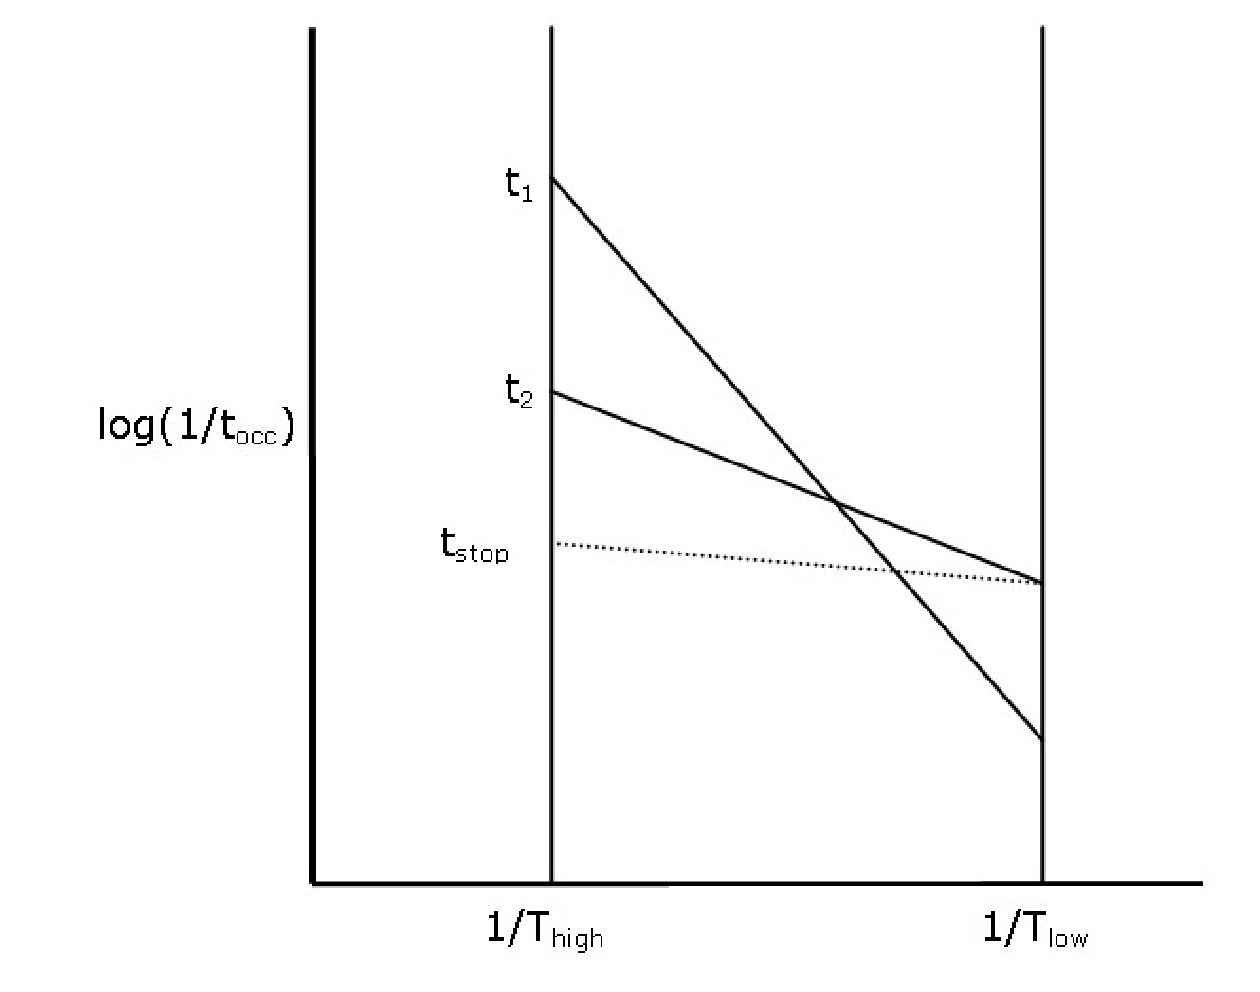
\psfig{file=TAD.ps,height=6cm}}
\end{center}
\caption{Basic TAD Theory\label{tadfig}}. 
Plot of $log(1/t)$ vs. $1/T$ for the TAD method. Simulations at high
temperature locate transitions indicated as $t_1$ and $t_2$ with $t_1$
occurring first (time increases in a downward direction on this
plot). Extrapolation to low temperature using equation
\ref{tad2} shows that these transitions would have occurred in reverse
order. If no other transitions occurred, $t_2$ would be the observed
low temperature transition in an MD simulation. The dotted line
indicates a possible hypothetical transition that just precedes
$t_2$ at low temperature. Its high temperature intercept is calculated
according to the criterion of Voter {\em et al.} \cite{voter-00a}
which gives the estimated stopping time for the simulation.

~
\hrule
\end{figure}

The characteristics of the method are as follows, in which it is
assumed that the kinetic properties of a system at the temperature
($T_{low}$) are required. 
\begin{enumerate}
\item The starting structure (state A) is energy minimised to provide a
reference structure (hereafter called the reference state) against
which later structures may be compared to determine any structural
transitions.
\item The system is simulated at high temperature ($T_{high}$)
and halted at regular intervals (called a `TAD block') to energy
minimise the structure to construct a reference state. This is
compared with the existing reference state to determine if a
structural transition (to state B) has occurred. A transition is
deemed to have occured if one or more atoms are displaced by more than
a preset distance (the `catch radius'). If a transition is
detected, a NEB calculation is initiated, using the two reference
structures, to find the activation energy ($E^{*}$).
\item Next a determination of the transition time ($t_{occ}^{high}$) is made.
As with BPD the occurrence time of the transition ($t^{high}_{occ}$)
is determined by checking back from the detection of the transition
through past configurations saved at regular intervals (which are
saved at intervals much less than a TAD block).  Each saved
configuration is energy minimised and compared with the reference
state structure until the first occurrence of the new state is
found. This provides a reasonable accuracy on the transition time,
somewhat better than using the end time of the TAD block in which the
transition occurred. 
\item The time $t_{occ}^{high}$ is extropolated to the
corresponding time of occurrence ($t_{occ}^{low}$) at $T_{low}$.  
This is done by combining equations (\ref{arrhenius})
and (\ref{tad1}) and taking the logarithm:
\begin{equation}
\log\left\{\frac{t_{occ}^{low}}{t_{occ}^{high}}\right\}=
\log\left\{\frac{k^{high}}{k^{low}}\right\}=-\frac{E^{*}}{k_B}
\left\{\frac{1}{T_{high}}-\frac{1}{T_{low}}\right\}. \label{tad2}
\end{equation}
See figure \ref{tadfig} for an indication of how the extrapolation
works. 
\item The system is returned to state A and the simulation recommenced. 
Returning the system to its original state means resetting the atomic
coordinates to a structure in the starting basin and resetting the
velocities according to a Boltzmann distribution, while retaining the
total system energy of the original state.  The simulation is
continued to obtain information on other transitions (to states C, D,
E etc) that may occur from state A. This is a key difference from the
BPD method.
\item A determination of the simulation `stopping time' ($t_{stop}$)
is made (see below). When the simulation reaches the calculated
stopping time, it is terminated.
\end{enumerate}

When the simulation has ended, the transition with the shortest
determined occurence time ($t_{occ}^{low}$) at $T_{low}$ indicates the
state to which the system would have transformed in a molecular dynamics
simulation at that temperature. This new state becomes the starting
point for a new high temperature simulation of the system, exploring
transitions from this state to futher new states. 
By this procedure, after sufficient sampling of states, the true low
temperature evolution of the system may be determined.

The `stopping time' mentioned above is the time at which the high
temperature simulation is halted. Ideally this is defined with a high
probability that no more significant transitions will be found.  This
is determined from the history of the TAD simulation itself. Voter
{\em et al.} provided a prescription of this \cite{voter-00a}. It
begins by defining, for a supposed undiscovered escape route, a very
small probability ($\delta$) that after the time $t_{stop}$ the system
is still in state A. This probability must chosen small enough to give
confidence that the awaited transition has had sufficient time to
occur. $\delta$ may be determined from
\begin{equation}
\delta=\int_{t_{stop}}^{\infty} k~\exp(-kt)~dt
\end{equation}
from which it follows that
\begin{equation}
\log\left (\frac{1}{\delta}\right )=t_{stop}k.
\end{equation}
and hence combining this with (\ref{arrhenius}):
\begin{equation}
\log\left (\frac{1}{\delta}\right
)=t_{stop}\nu_{min}\exp(-E^{*}_{min}/k_BT_{high})
\end{equation}
where $\nu_{min}$ and $E_{min}^{*}$ are the prefactor and activation
energy respectively of the supposed undiscovered escape
route. Rearranging this gives
\begin{equation}
T_{high}~\log\left (\frac{\log(1/\delta)}{t_{stop}\nu_{min}}\right )=
-\frac{E^{*}_{min}}{k_B} \label{tad3}
\end{equation}

The supposed undiscovered escape route is one which may possesses a
low temperature occurrence time that is less than the current working
minimum ($t_{occ}^{min}$). The right side of (\ref{tad3}) may be
approximately determined using equation (\ref{tad2}) if it assumed
that the largest observed value of $t_{occ}^{high}$ is close to
$t_{stop}$ and the lowest possible low temperature time is close to
$t_{occ}^{min}$ (see figure \ref{tadfig}). Combining the two equations
and rearranging gives
\begin{equation}
t_{stop}=\left (\frac{\log(1/\delta)}{\nu_{min}}\right )
\left (\frac{t_{occ}^{min}\nu_{min}}{\log(1/\delta)}\right )^{T_{low}/T_{high}}.
\end{equation}

Voter \cite{voter-00a} argues that $\nu_{min}$ is commonly of the order
$10^{12}\sim 10^{13}$ $s^{-1}$ (or $1 \sim 10$ in DL\_POLY units) and
suggests $\delta=0.001$ as a working value. These represent practical
working values for approximating $t_{stop}$.

\subsection{Running a TAD Simulation}

This section describes the procedure for running a TAD simulation.
The reader will notice some resemblance to the BPD procedure described
in section \ref{BPD}. This is intentional for operational reasons, but
the reader should always be alert to the key differences between the two.

We recommend the following procedure.
\begin{enumerate}
\item Run a normal simulation of the system at the (high) temperature 
($T_{high}$) needed to perform the TAD simulation. Make sure the
system behaves itself before moving to the next stage (and doesn't
melt, for example). Retrieve the REVCON file and rename it as CONFIG
for the TAD run. In principle this equilibration can be skipped and a
TAD simulation started right away (with a suitable equilibration
period at the start), but it is probably wiser to do this stage
beforehand and make sure the system behaves properly at this
temperature.
\item Set up the TAD simulation using the directives in the CONTROL 
file as follows:
\begin{enumerate}
\item Set the {\bf tad} directive followed by records defining the
operating conditions:
\item Define the energy units for the TAD parameters e.g. \newline
 {\bf units} {\em s}\newline where {\em s} is one of {\em eV, kcal, kJ
 or K}, signifying electron volts, kilo cals per mole, kilo joules per
 mole or Kelvin, respectively. No {\bf units} directive means DL\_POLY
 internal units apply. Forces are in chosen energy units per Angstrom.
\item Set the size of the simulation TAD block i.e. the number of
  time steps between structure optimisations. e.g. \newline
  {\bf num\_block} 500.
\item Set the number of configurations between each write of a tracking
  configuration file. This should be an integer divisor of the TAD
  block number. e.g. \newline
  {\bf num\_track} 10.
\item Set the blackout period (in time steps) following a transition
  detection. e.g. \newline
  {\bf blackout} 200.\newline
  A blackout period is intended to stop the program recording
  transitions that are correlated with a previous one. These are
  classified as `ignored transitions'
\item Set the `catch radius' i.e. the minimum distance 
  in Angstroms any atom may be displaced in the minimised structure
  before it is recorded as a transition e.g. \newline
  {\bf catch\_radius} 3.0.
\item Set the NEB spring constant (in specified energy units per $\AA^2$). 
       e.g. \newline {\bf neb\_spring} 1000.0 (in DL\_POLY units).
\item Set the reliability factor for the high temperature 
 simulation. For input purposes this is defined as the ratio 
 $\log(1/\delta)/\nu_{min}$ (see above) e.g. \newline
 {\bf deltad} 0.001.
\item Set the low temperature ($T_{low}$) for the TAD method (i.e. 
 the temperature for which the results are needed, in Kelvin) e.g. \newline
 {\bf low\_temp} 30.0.
\item Select a minimisation option.  e.g. 
 \newline {\bf keyword} {\em tol}.\newline Where {\bf keyword} is one of
 {\bf force, energy, position} and {\em tol} is the convergence
 tolerance.  (The recommended tolerance for {\bf force} option is 1.0
 in DL\_POLY units.) e.g. \newline {\bf force} 1.0.
\item Close the TAD definition with the directive \newline {\bf endtad}
\end{enumerate}
\item Set other CONTROL file keywords as follow:
\begin{enumerate}
\item The simulation temperature (i.e. the `high' temperature
$T_{high}$ for the TAD method) using the {\bf temp} directive.
\item Select the {\bf restart noscale} option if the CONFIG file was
pre-equilibrated, otherwise leave out the {\bf restart} keyword
altogether.
\item Set the length of the simulation required ({\bf steps}) and 
 the equilibration period ({\bf equil}) (both in time steps). The
equilibration can be short if the system was pre-equilibrated.
\item In setting the job {\bf close time}, it is recommended to set the number
  to at least 500 times the clock time it takes to do one normal MD
  time step. This is to prevent the program running out of time during
  a structural minimisation. The timing information for this may be
  taken from the previous equilibration run.
\item Set the remaining CONTROL keywords as were defined for the initial
  equilibration simulations.
\end{enumerate}
\item Before starting the TAD simulation, use the UNIX `mkdir' command to
   make the following empty directories: 
\begin{itemize}
   \item {\em BASINS} - to receive any new structures found
   \item {\em TRACKS} - to store the tracking configurations
   \item {\em PROFILES} - to store any transition pathways found by NEB calculation
\end{itemize}
   If the directories {\em BASINS, TRACKS} and {\em PROFILES} already
   exist then carefully archive the data before deleting the
   contents. Do not empty these directories if continuing (restarting)
   the simulation in the original starting basin. The information in
   these directories is still `live' in this case. Further information
   on these files can be found in section \ref{hypfiles}.
\item Run the TAD simulation. This will perform a simulation at the
  (high) temperature requested, checking for structural transitions at
  the intervals specified. Each time it finds a structural
  transition, it will record the new state, determine the activation
  energy, transition pathway and stopping time, then revert back to
  the starting basin and continue.
\item When the simulation ends, proceed as follows.
\begin{enumerate}
\item Check the EVENTS file to see if any structural transitions
  have been obtained. Each event is represented by a single record and
  transitions are flagged with the keyword TRA at the start of
  the record. Use unix `grep' to locate these entries. No observed
  transitions indicates either a longer simulation is necessary, or
  a higher temperature simulation should be considered.
\item Check that the simulation was sufficiently long to guarantee all
  high temperature transitions have been found that are compliant with
  the specified reliability ({\bf deltad}). The estimated stop time derived
  from this factor appears as the last entry of the TRA record in the
  EVENTS file.
\item If the simulation stop time has not been reached, the job must be
  restarted from the REVCON, REVIVE and HYPRES files (renaming them
  as CONFIG, REVOLD and HYPOLD for the purpose), and continued
  until the stop time has been reached. After the simulation finally stops,
  a new simulation can be started from the basin file obtained from
  the earliest (shortest extrapolated time) low temperature
  transition. See section \ref{tadrestart} for more information on
  restarting a TAD simulation.
\item Use the DL\_POLY Java GUI to plot the system energy and temperature
  for the whole of the simulation. Apart from the equilibration period,
  these should hold their values within normal thermodynamic fluctuation, 
  even if transitions have occured. If they do not, the system probably 
  has not been equilibrated adequately to begin with, in which case
  start the simulation again. (See sction \ref{tadrestart}.)
\item Check that all the new states the program found are in 
  the {\em BASINS} directory. Note that there may be fewer new states
  than the number of transitions observed because some transitions
  may end in the same basin more than once, so a new state is not
  stored in this case. Examine them using the DL\_POLY Java
  GUI. There may be signs of imperfect minimisation (atoms not quite on
  lattice sites etc) but this is normal at this stage. Corrective
  action can be taken later (see section \ref{tidyup}).
\item Check that the profiles for all the reported transitions have been
  written in the {\em PROFILES} directory. These record the change in
  configuration energy as a function of reaction coordinate.  Plot
  these using the DL\_POLY Java GUI. Use the GUI `spline' option to
  get a better idea of what the profiles look like. Take special note
  of any double (or multiple) maxima. The transition is considered to
  end at the first minimum in these cases. A basin file for the first
  intermediate state is written to the BASINS directory.
\end{enumerate}

\subsection{Restarting a TAD Simulation}
\label{tadrestart}
It may be necessary to restart a TAD simulation for a number of reasons.
\begin{enumerate}
\item The earliest low temperature transition
  from the current basin has been found and the user now wants to
  investigate transitions from the new basin. This basin corresponds
  to that which a molecular dynamics simulation would have reached
  first at the low temperature. In which case users should save their
  data from the first study and commence the simulation from the new
  basin exactly as in the previous study i.e. renaming the appropriate
  basin CFGBSNnn file as CONFIG. Once again an initial equilibration of the
  system to high temperature is recommended. This is not strictly a
  restart of an unfinished simulation, but the start of a new one
  which is part of a TAD series.
\item The previous simulation ended but did not record any transitions. 
  In this case it is advised to start the simulation afresh, using a
  higher operating temperature than before. 
\item The previous simulation ended without crashing and recorded 
  some transitions but did not reach the required stop time. In this
  case simply restart the program as for a normal DL\_POLY
  continuation run - using the REVCON, REVIVE and HYPRES files
  (renamed CONFIG, REVOLD and HYPOLD) and using the unqualified {\bf restart}
  directive in the CONTROL file. (Remember to increase the number of
  required time steps if necessary.)
\item The previous simulation crashed. If this means a crash for unknown
  reasons, then the situation may be unrecoverable (as with any
  unexpected DL\_POLY crash). Try to locate the problem and fix it. If
  however the simulation arrived at this end point due to a time-out
  error, then there is hope. It may be possible to restart from the
  last REVCON, REVIVE HYPRES files, presuming they are uncorrupted and
  have the same time stamp. Be aware that such a restart may cause
  data duplication in other files, such as STATIS, EVENTS, {\em
  BASINS}, {\em PROFILES} and HISTORY, and the user should remove such
  a possibility by editing or sometimes even removing the files before
  restart. The objective is to remove any entries in these files that
  occured after the restart files were written. It is therefore
  important to determine what was going on when the program
  crashed. With TAD it may be found that the time-out error is most
  likely to happen during a NEB calculation or a structure
  optimisation. In which case it will be hard work deciding what needs
  to be patched up before continuing, though the time stamp of the
  restart files is still the crucial factor. This situation is best
  avoided in the first place by giving the code a generous `close
  time' in the CONTROL file, so that these optimisation tasks have a
  chance to complete before the axe falls.
\end{enumerate}
\end{enumerate}

\subsection{Things to Be Aware of when Running  TAD}

\begin{enumerate}
\item Choose the `catch radius' carefully, where possible basing it on
  nearest neighbour distances obtained form the parent crystal. A
  consequence of using too large a catch radius is that transitions
  that require a short hop in atom positions may be missed during a
  run. Such misses make it difficult to reconstruct the reaction path
  and, in particular, cause the NEB calculation to crash, since there
  is no simple path between the reference structures.
\item The user may sometimes observe successive transitions into the same 
  state. If a transition to an already visited state occurs it is
  indicated with the flag TRR (repeat transition) in the EVENTS
  file. Such repeated transitions are normal but if they occur in
  succession it implies that there is some correlation creeping into
  the resetting of the system back into the starting state. This
  however is harmless as the accumulated simulation time is reset back
  to the restart state after each transition and so does not affect
  the time of the later transition to a new state.
\item Note that in a TAD simulation the reference state is always 
  the same. The reference state does not `follow' the diffusion path as
  it does in BPD.
\item It is useful to determine which atoms have relocated during a
  transition. The program bsncmp.f in the {\em  utility} directory 
  may be used for this purpose. It is designed to compare start and 
  end configurations in the {\em BASINS} subdirectory and list the 
  atoms that have changed location.
\end{enumerate}

\section{\D{} Hyperdynamics Files}
\label{hypfiles}

The \D{} BPD and TAD options generate a (potentially large) number of
files in addition to those normally produced (and described in Chapter
4). Some are sufficient in number to warrant creation of additional
sub-directories of the DL\_POLY {\em execute} sub-directory. These
files are as follows.

\begin{enumerate}
\item HYPRES - the hyperdynamics restart file, which stores 
(unformatted) data to permit continuation of an unfinished BPD or TAD
simulation. It is created in the {\em execute} sub-directory. This
file becomes the HYPOLD file, which is used in restarting a BPD or TAD
simulation.
\item EVENTS - a summary of events that have occurred in the
course of a hyperdynamics simulation - one record per event. It is
generated in the {\em execute} sub-directory.
\item CFGBSNnn - a `basin' file, which contains the coordinates of each
distinct state \D{} has found during the BPD or TAD run. nn is an integer
rising from 0 to 9999. All such files are generated in the {\em
execute/BASINS} sub-directory.
\item PROnn.XY - a `profile' file, which is a list of the reaction 
coordinate and configuration energy of each bead in the converged NEB
calculation. nn is an integer rising from 0 to 9999. All such files are
generated in the {\em execute/PROFILES} sub-directory and are plotable
XY files.
\item CFGTRAnn - a configuration file used to interpolate when a
transition has occured. nn is an integer rising from 0 to 9999.
All such files are generated in the {\em execute/TRACKS} sub-directory.
\end{enumerate}
These files are described in further detail below.

\subsubsection{The HYPRES and HYPOLD Files}

The HYPRES and HYPOLD files are unformatted (i.e. not human readable)
and are {\em restart files} for BPD or TAD runs of \D{}. The HYPRES file
is produced by the program at regular intervals during the program run
and also at the end of a run. It must subequently be renamed HYPOLD to
be read by \D{} when the simulation is recommenced. The user does not
need to know the contents of these files, but for the curious it can
be said that they contain current file numbers for the {\em BASINS},
{\em TRACKS} and {\em PROFILES} directories; the structural
differences between the current reference basin and any new basins
found (TAD only); and the atomic coordinates of the current basin
taken at the last check point (such as the end of the last BPD orTAD
block).

\subsubsection{The EVENTS File}
\label{eventsfile}
\index{EVENTS file}

The EVENTS file is a text file that reports the results of actions
taken by the hyperdynamics routines. Each record in the file specifies a
particular kind of event. The possible events described are as
follows. (Note that the real variables specified in this file are
in units specified by the user.)
\begin{enumerate}
\item Blackout period reset: {\bf BLK n1 n2} \newline
where 
\begin{itemize}
\item n1 is the time step at which a blackout period was initiated;
\item n2 is time step at which the new blackout period will end.
\end{itemize}
TAD only.
\item Equilibration period reset: {\bf EQL n1 n2} \newline
where 
\begin{itemize}
\item n1 is the time step at which the equilibration period was reset;
\item n2 is time step at which the new equilibration period will end.
\end{itemize}
\item Minimisation completed: {\bf MIN n1 n2 n3 n4 r1 r2 r3} \newline
where
\begin{itemize}
\item n1 is the time step at which the minimisation commenced (integer);
\item n2 is number of cycles required by the minimiser to converge (integer);
\item n3 is the BPD/TAD block for which the minimisation took place (integer);
\item n4 is the optimisation convergence criterion key: 0 for forces,
1 for energy, 2 for position (integer);
\item r1 is the convergence tolerance used by the minimiser (real);
\item r2 is the energy of the minimised configuration (real);
\item r3 is the the convergence actually achieved by the minimiser (real).
\end{itemize}
Users should note that a final convergence value (r3) greater than the
convergence criterion (r1) indicates incomplete convergence.
\item Nudged Elastic Band completed: {\bf NEB n1 n2 n3 n4 r1 r2} \newline
where
\begin{itemize}
\item n1 is the time step at which the NEB calculation commenced (integer);
\item n2 is number of cycles required by the NEB calculation to converge (integer);
\item n3 is the maximum allowed number of cycles (integer);
\item n4 is the number of `beads' in the NEB chain (integer);
\item r1 is the energy of the home basin (starting state) configuration (real);
\item r2 is the energy of the end basin (new state) configuration (real);
\end{itemize}
Users should note that when n2 and n3 are equal, this implies that
convergence of the NEB chain has not been achieved. Note also that the
characteristics of the reaction path are given by the subsequent {\bf
TRA} event (below).
\item Transition detected: {\bf TRA n1 n2 n3 n4 r1 r2 r3 r4} \newline
where
\begin{itemize}
\item n1 is the time step at which the transition was first detected (integer);
\item n2 is the home basin (starting state) of the transition (integer);
\item n3 is the new basin (ending state) of the transition (integer);
\item n4 is the number or turning points in the transition profile (integer);
\item r1 is the activation energy obtained from the NEB calculation (real);
\item r2 is the observed transition time (real);
\item r3 is the calculated extrapolated transition time (real);
\item r4 is the calculated stopping time (real, TAD only);
\end{itemize}
\item Transition ignored: {\bf TRI n1} \newline
where
\begin{itemize}
\item n1 is the time step at which a transition was detected, but
ignored because it was during an equilibration or blackout period
(integer). 
\end{itemize}
TAD Only.
\item Transition repeated: {\bf TRR n1 n2 n3} \newline
where
\begin{itemize}
\item n1 is the time step at which a transition was detected, but
it was identified as a repeat and no further analysis was underatken
(integer);
\item n2 is the identity of the home basin (integer);
\item n3 is the identity of the new basin (integer);
\end{itemize}
TAD Only.
\end{enumerate}

\subsubsection{The CFGBSNnn Files in the {\em BASINS} Directory}
\label{cfgbsn}
\index{BASINS directory}
\index{CFGBSNnn file}

A CFGBSNn file is a text file containing the energy minimised
structure of a basin found during the BPD or TAD
simulation. The number nn rises from 0 to 9999. Internally the format
of the file is the same as a CONFIG file (see section
\ref{configfile}), though it does not normally contain velocity or 
force data.

\subsubsection{The CFGTRKnn Files in the {\em TRACKS} Directory}
\index{TRACKS directory}
\index{CFGTRKnn file}

The CFGTRKnn files have exactly the same format as the CFGBSNnn
files. The files do not however contain energy minimised structures.
These files represent consecutive structures written at user defined
intervals during the simulation. The interval ({\bf num\_track} see
above) is an integer divisor of the number of steps in a BPD or TAD
block ({\bf num\_block}) and the number nn in the file name is modulo
{\bf max\_track}, where {\bf max\_track}={\bf num\_block}/{\bf
num\_track}. Thus after {\bf num\_block} time steps from the
simulation start, there are always {\bf max\_track} configurations to
search back over to locate the time of a transition. nn is an integer
ranging from 0 to {\bf max\_track}.

\subsubsection{The PROnn.XY Files in the {\em PROFILES} Directory}
\index{PROFILES directory}
\index{PROnn.XY file}

\index{hyperdynamics!reaction path}
The PROnn.XY files tabulate the converged configuration energies of the
beads in a NEB calculation, as a function of the reaction coordinate
linking the beads. nn is an integer ranging from 0 to 9999.

The reaction coordinate is the path distance ($S_{n}$) between the
structure of the reference state and the structure of a converged NEB
bead and is defined here as: 
\begin{equation}
S_{n}=\sum_{i=1}^{n}\left [(\vek{R}^{N}_{i}-\vek{R}^{N}_{i-1})^{2}\right ]^{1/2},
\end{equation}
where $\vek{R}^{N}_{i}$ is a 3N dimensional vector defining the structure
(N is the number of atoms) and $n$ ranges from $2$ to bead number
$N_{neb}$ in the NEB chain.  Note that the reaction path does not
usually represent a straight line in the 3N dimensional space.  The
file PROnn.XY presents two columns of numbers: the first is the
reaction coordinate and the second is the configuration energy of the
bead. Both are expressed in \D{} units. The configuration energy for the
first bead (at $S_{n}=0$) is the energy of the reference state.

Normally the PROnn.XY file reveals a single maximum in configuration
energy as the reaction coordinate increases. However in some instances
more than one maximum may be obtained. The user should note that in these
instances \D{} will take the configuration closest the first minimum
and optimise it independently to define the true destination of the
transition from the reference state.

\section{Tidying Up the Results of a Hyperdynamics Simulation}
\label{tidyup}

\subsection{Refining the Results}

A completed BPD or TAD simulation will provide a number of basin files
defining the minima of new structures discovered, together with the
associated profile files describing the energy path between these
structures. These are the data that are needed to reconstruct the
diffusion path in the original system.

However, at this stage there are still some approximations in the
results, which arise from the chosen tolerances in the energy
minimisation of the structures and the NEB calculations. To offset
these, the following refinements are recommended.
\begin{enumerate}
\item Take each of the basin structures derived from the BPD or TAD 
  simulation and perform a further structural optimisation with
  DL\_POLY, using more exacting convergence tolerance. For example
  using a force tolerance of 0.01 (DL\_POLY units) in place of the
  recommended 1.0 used in the BPD and TAD procedures. This will
  provide more accurate reference structures.
\item Using the accurately minimised structures in place of the original
  basins, use the NEB option in DL\_POLY to recalculate the transition
  path between the reference states. Once again a more exacting
  tolerance may be used, but beware that the NEB calculation may not
  converge at all if the tolerance is too exacting. It is far less
  stable in this respect than the ordinary structural
  optimisation. Note that the tolerance for the overall NEB
  minimisation is set internally in \D{} to be a factor of 10 larger
  than that for the minimisation alone. The result of these
  refinements should be a better estimate of the activation energy and
  low temperature transition time.
\end{enumerate}

For TAD simulations the activation energy obtained from the refined
structures can be used together with the simulated high temperature
transition time to recalculate the low temperature transition time
from equation (\ref{tad2}). Note this may alter the original low
temperature diffusion path, so be alert to this possibility and change
the starting basin for any subsequent simulation. These refinements
have no impact on the BPD simulations other than to improve the
quality of the calculated kinetic properties.

\subsection{Treatment of Multiple Maxima in the Reaction Path}

\index{hyperdynamics!reaction path}
The NEB calculations that occur while the BPD or TAD simulations are
running may sometimes report a multiple maximum on the reaction path
(see the {\bf TRA } entry for the EVENTS file in section
\ref{eventsfile}). More than two maxima is probably indicative of
problems with the NEB convergence and should be regarded with
suspicion, but obtaining two maxima is a real possibility. In such
cases \D{} stores both the end structure of the NEB chain and the
structure corresponding to the first minimum in the energy profile
along the reaction path, but it does not record the activation
energies beyond the first peak.

A BPD simulation requires a complete description of the potential
energy surface kinetics so determination of the second activation
energy and the corresponding transition time is essential. After
recording the transition, the subsequent dynamics correctly starts
(for BPD) from the final state of the double transition, but the loss
of information is ignored. A NEB calculation is therefore necessary to
determine the lost details.

For TAD objective is to find the escape route for a transition from
the starting state and halting the analysis of the reaction path at
the first minimum is sufficient to define the escape. The intermediate
state provides a valid possible basin for further study of the
kinetics of the system. This is sensible if the two peaks on the
reaction path are of similar magnitude. However it is quite possible
that the second peak is much higher or much lower than the first. The
first of these possibilities means that choosing the first minimum as
the starting basin for a new simulation will most likely consistently
return the system to the original starting state. The second
possibility suggests that the second state on the reaction path is a
better option for the next phase of the study. To decide between these
possibilities it is necessary to determine the activation energy of
the second peak. Thus in both BPD and TAD, when a multiple maximum is
found on the reaction path, a NEB calculation is needed to complete
the path analysis.

See the following section \ref{nebrun} for details.

\section{Running a Nudged Elastic Band Calculation}
\label{nebrun}
\index{hyperdynamics!NEB}
Running an independent NEB calculation may be necessary to improve
the accuracy of the calculated activation energy, or to determine the
activation energy in transitions not fully evaluated when they
occurred in a BPD or TAD simulation - due to the occurrence of a
multiple maximum on the reaction path.\index{hyperdynamics!reaction path}

To run a NEB calculation with \D{} it is first necessary to identify the
start and end basins among the CFGBSNnn files in the BASINS directory
described in section \ref{cfgbsn}. From the information provided in
the EVENTS \ref{eventsfile} file it should be possible to decide which
files are needed. The user then needs to modify the CONTROL file in
the following way.
\begin{enumerate}
\item Remove any directives for the {\bf bpd} or {\bf tad}
options. Directives for the integration algorithm ({\bf integrator}) or
ensemble ({\bf ensemble}) should also be removed.
\item The directive for the NEB option should be inserted: \newline
{\bf neb} {\em n} \newline
where {\em n} is the number of NEB calculations required.
\item On the record following the {\bf neb} directive, a list of 
{\em n} starting basins  should be given e.g.\newline
{\bf basin\_1} 1 1 1 2 3 \newline
Meaning the 5 required NEB calculations start from basin files
CFGBSN0001, CFGBSN0001, CFGBSN0001, CFGBSN0002 and CFGBSN0003. Up to
10 NEB calculations are permitted.
\item On the second record following the {\bf neb} directive, a list of 
{\em n} final basins should be given e.g.\newline
{\bf basin\_2} 2 3 4 3 4 \newline
Meaning the 5 required NEB calculations are between basins 1 - 2, 1
- 3, 1 - 4, 2 - 3 and 3 - 4 in this example.
\item Define the energy units for the BPD parameters e.g. \newline
{\bf units} {\em s}\newline where {\em s} is one of {\em eV,
kcal, kJ or K}, signifying electron volts, kilo cals per mole,
kilo joules per mole or Kelvin, respectively. No {\bf units}
directive means DL\_POLY internal units apply. Forces are in
chosen energy units per Angstrom.
\item Next set the NEB spring constant (in specified energy units per $\AA^2$). 
e.g. \newline {\bf neb\_spring} 1000.0 (in DL\_POLY units).
\item Select a minimisation option.  e.g. 
\newline {\bf force} {\em key tol}.\newline 
Where {\em key} is one of {\em force, energy, position} and {\em
tol} is the convergence tolerance.
\item Close the NEB definition with the directive \newline
{\bf endneb}
\end{enumerate}

\subsection{Things to Aware of when Running a NEB Calculation}

\begin{enumerate}
\item Note that the NEB calculation assumes that the basin files for
the start and end states are in the BASINS directory and that \D{} is
being run from the {\em execute} directory, where the DLPOLY.X
executable is located. Needless to say, if these files are placed
anywhere else, the calculation will fail. 
\item Note also that the NEB
calculation places the reaction path profile for a given pair of
states in the PROFILES direction with the file name PRXnn.XY, where {nn}
is a {\em negative} number that is compounded from the identities of the
start ($n_1$) and end states ($n_2$) thus: $nn=-(100*n_1+n_2)$.
\item It is important to be sure that the start and end states
represent real, observed transitions in the BPD or TAD simulation. The
danger here is using two structures that are not mechanistically
close. If this is not the case, the NEB calculation is unlikely to
converge, as there will be no simple path (with preferably a single
energy maximum) between the start and end states.
\item When running an NEB calculation to improve the
accuracy of the activation energy a more stringent tolerance must be
set. For example the recommended value for the force tolerance is
normally 1.0 (in DL\_POLY units), but values one or two orders of
magnitude less may be tried. It should be noted however that before
the NEB calculation is run, the configurations representing the start
and end configurations must first be minimised to the accuracy
required by the new tolerance, by using the \D{} {\bf optim}
option. These optimised structures must be returned to the BASINS
directory with the same file numbers as the original CFGBSN files.
\end{enumerate}


